%%%%%%%%%%%%%%%%%%%%%%%%%%%%%%%%%%%%%%%%%%%%%%%%%%%%%%%%%%%%%%%%%%%%%%%%%%%%%%%%
% Soutenance de projet - Fichier modèle pour présentations Beamer
%%%%%%%%%%%%%%%%%%%%%%%%%%%%%%%%%%%%%%%%%%%%%%%%%%%%%%%%%%%%%%%%%%%%%%%%%%%%%%%%
\documentclass{beamer}
\usepackage[utf8]{inputenc}
\usepackage[francais]{babel}
\usepackage[T1]{fontenc}
\usepackage{textcomp}
\usepackage{relsize}
\usepackage{amssymb}
\usepackage{framed}


%%% THÈME TORINO AVEC MINIFRAMES MODIFIÉES - NÉCESSITE FICHIERS SPÉCIAUX
\usetheme[pageofpages=sur,% String used between the current page and the
                         % total page count.
          alternativetitlepage=true,% Use the fancy title page.
          titlepagelogo=logo,% Logo for the first page.
          titleline=true,
          watermark=watermark,% Watermark used in every page.
          watermarkheight=100px,% Height of the watermark.
          watermarkheightmult=4,% The watermark image is 4 times bigger
                                % than watermarkheight.
          ]{Torino}
\useoutertheme[subsection=true]{miniframes2}
\usecolortheme{freewilly}
%%% FIN DU SECOND THÈME

% nouvelle commande pour un joli nom
\newcommand{\nom}[1]{\textsc{#1}}

% commande pour une zolie ligne
\newcommand{\ligne}[1][1pt]{
  \par\noindent
  \rule[.5ex]{\linewidth}{#1}\par}

% \0
\newcommand{\slz}{$\backslash0$}

% commande pour un message réseau
\newcommand{\netmessage}[5]{\small \begin{framed}
\texttt{Message} \emph{#1} \texttt{- #2 - #3 $\rightarrow$ #4}\\\noindent
\rule{\linewidth}{0.4pt}

\footnotesize\noindent\texttt{#5}

\end{framed}}

%%% TITRE DE PAGE
\title{Capture d'activité système pour PIGA-SYSTRANS}
\author{Dimitri~Gressin \and Timothée~Ravier}
\institute{ENSI de Bourges}
\date{\today}

%%% POUR AVOIR UN PLAN QUI S'AFFICHE QUAND ON CHANGE DE SOUS-SECTION
\AtBeginSection[ ]
{
 \begin{frame}<beamer>
   \frametitle{Plan}
   \tableofcontents[currentsection]
  \end{frame}
}
\NoAutoSpaceBeforeFDP

\begin{document}

%%% LA PAGE DE TITRE, ON PEUT Y APPLIQUER DES OPTIONS COMME INSTITUTE CI-DESSOUS
{
	\framenumberoff
	\watermarkoff
	\institute{École Nationale Supérieure d'Ingénieurs de Bourges} % Vire le champ institut sur cette page
	\begin{frame}
	\titlepage
	\end{frame}
}


\section{Introduction}
\begin{frame}
\frametitle{Présentation du sujet}
\begin{enumerate}
	\item Intercepter les appels systèmes au niveau de l'espace noyau
	\item Récupérer des informations telles que PID, fichiers ouverts, socket créée, etc.
	\item Envoyer ces informations dans l'espace utilisateur au démon contextd
	\item Retourner la réponse de contextd au noyau pour débloquer l'appel système
\end{enumerate}
\end{frame}

\section{Systemtap}
\begin{frame}
\frametitle{Systemtap}
\begin{center}
	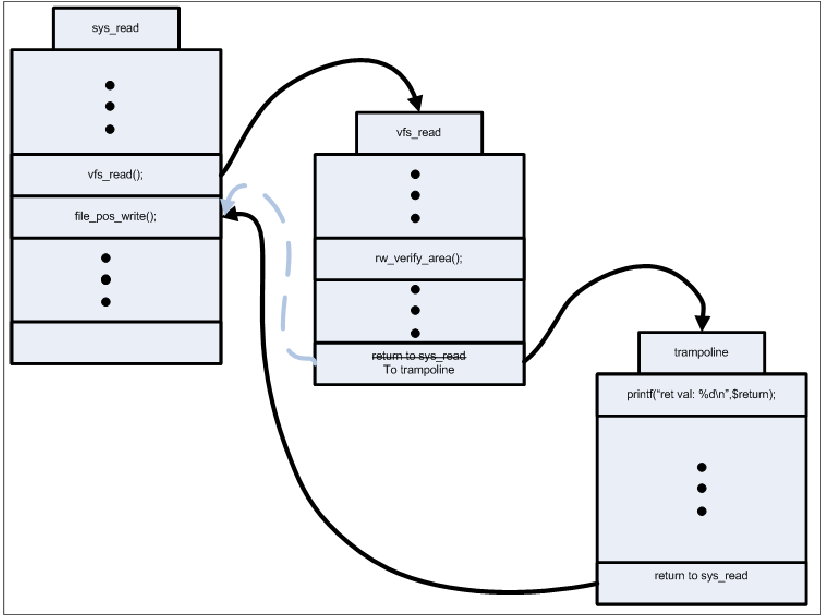
\includegraphics[scale=0.25]{kretprob.png}
\end{center}
\end{frame}

\begin{frame}
\frametitle{Systemtap}
\begin{itemize}
	\item Les scripts sont exécutés après les appels systèmes
	\item Impossibilité de suspendre un appel système
	\item Les données accessibles sont inexploitables
\end{itemize}
~\\
\textbf{Systemtap ne répondait absolument pas à nos besoins}

\end{frame}

\section{Linux Security Modules}
\begin{frame}
\frametitle{}

\end{frame}


\subsection{Objectifs suivants}
\begin{frame}
\frametitle{}

\end{frame}

\section{Conclusion}
\begin{frame}
\frametitle{}

\end{frame}

\end{document}
